\chapter{Hardware}
%http://samurai1967.dyndns.org/avr-net-io.html
%http://www.fhemwiki.de/wiki/AVR-NET-IO
%http://www.mikrocontroller.net/articles/AVR_Net-IO_Bausatz_von_Pollin
\section{AVR Net-IO-Board}
\begin{figure}[h]
\centering
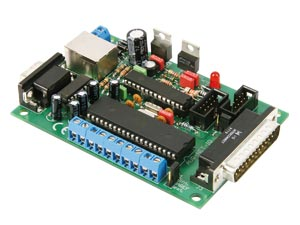
\includegraphics[width=7.5cm]{content/pictures/avr-net-io.jpg}
\caption{AVR-NET-IO - Pollin GmbH}
%http://www.pollin.de/shop/dt/MTQ5OTgxOTk-/Bausaetze_Module/Bausaetze/Bausatz_AVR_NET_IO.html
\label{fig:B3}
\end{figure}

Auf dem AVR Net-IO-Board sind der Webserver und die Webseite gespeichert. Die
verschiedenen Pins lassen sich darüber ansteuern und manipulieren.
Die Platine des AVR-Net-IO ist für den einfachen Anschluss der Externen
Anwendungen gedacht. Der Fokus liegt hier, je nach verwendetem Anschluss Bord
nicht darauf eine optimale Gestaltung zu haben sondern die einzelnen Sensoren
eher lose an die Platine anzuschließen. Dies geschieht wie in der Elekronik oft
üblich über die Verwendung von Breadboards, blanke Steckbretter auf
denen Schaltungen konzipiert werden können. Deswegen haben die Analog zu Ditital
Wandler Schraub-Verbindungen und auch die im Handel verfügbare Anschlussplatine
für den 25 Poligen D-Sub Stecker hat Schraub-Verbindungen. Für die Demonstration
haben wir uns spezielle Schaltungen überlegt die an die einfach an die Externen
Anschlüsse das AVR-Net-IO Angeschlossen werden können. Die verteilung, Welcher
Pin an welchem Anschluss ist, kann dem dem Schaltplan entommen werden. (siehe
Anhang, Abbildung \ref{anh:schaltplan})

\subsection{Technische Daten}
\begin{itemize}
  \item Betriebsspannung 9V 
  \item Stromaufnahme ca. 190 mA
  \item 14 Digitale Ein/Ausgänge, 4 Digitale Eingänge
  \item 4 Analoge Eingänge
  \item ATmega644P Mikrocontroller
  \item integrierte ISP-Schnittstelle
\end{itemize}

\section{Mikrocontroller}
Das Team hatte zu Beginn einen ATmega32 Prozessor als Vorgabe. Dieser hat jedoch nur 32kB Flash Speicher. Nach ersten 
Feldversuchen wurde schnell klar, dass ein Speicher von 32kB nicht ausreichen wird, weshalb das Team auf einen ATmega644P 
ausgewichen ist. Dessen Speicherressourcen liegen bei 64kB und reichen für Webserver und Webseite aus, weshalb das Team 
nicht auf die größere Variante, den ATmega1284P ausweichen musste.\\ 
Anbei ein kleiner Vergleich der wichtigsten Bestandteile der 
drei Prozessoren. Weitere Informationen würden den Rahmen sprengen und können
bei Bedarf dem entsprechendem Datenblatt entnommen werden.

\begin{table}[H]
\begin{tabular}{|c|c|c|c|} \hline 
  Mikrocontroller & ATmega32 & ATmega644P & ATmega1284P \\ \hline 
  Flash & 32kB & 64kB & 128kB \\ \hline
  Pins & 44 & 44 & 44 \\ \hline
  Max. Operation Freq. & 16MHz & 20MHz & 20MHz\\ \hline
  Max. I/O Pins & 32 & 32 & 32 \\ \hline
\end{tabular}
\caption{Mikrocontroller im Vergeich}
\label{mikrocontroller}
\end{table}

\subsection{ENC28J60}

Der ENC28J60 ist der IEEE 802.3 kompatibe Netzwerk Contoller des AVR-Net-IO er
nimmt die externen Anfragen an und reicht diese an den ATMega weiter. Dabei ist
er an Port B des ATMegas Angeschlossen, dieser kann deswegen nicht für Ein- oder
Ausgaben verwendet werden.

\newpage
\section{Fuse Bits}
\label{chap:Fuse}

Die Fuse-Bits sind die Grundlegenden Einstellungen, mit denen ein
Mikrocontroller arbeitet. Sie müssen geändert werden, wenn ein anderer Taktgeber
gewünscht ist oder Schnittstellen de- oder aktiviert werden sollen.\\
\\
\fcolorbox{red}{white}{
	\parbox{\dimexpr \linewidth-2\fboxsep-2\fboxrule}{
		\textbf{Allgemeiner Hinweis:} Dieser Artikel kann die Recherche im Datenblatt
		nicht ersetzen, besonders bei abweichendem Mikrocontroller sind die Fuse-Bits
		oft anders gewählt. Mit dem Atmel Studio kann es vorkommen, dass man sich vom
		Mikrocontroller aussperrt. Ein zurücksetzen der Fuse-Bits kann mit AVRDUDE
		in diesem Fall versucht werden. Beschrieben wird dieser Vorgang im
		Benutzerhandbuch \ref{Chapt:Einrichten}
	}}\\
\\
In Tabelle \ref{fuses-names} werden die einzelnen Fuse-Bits zusammen mit ihrer
Bedeutung und dem entsprechendem Byte aufgelistet. Der Schlussendliche Fuse Wert
setzt sich aus zwei Byte zusammen, wobei eine 1 eine deaktivierte Eigenschaft und
eine 0 aktiviert Eigenschaft bedeutet. Kleinere Mikrocontroller besitzen nur ein
High (H) und ein Low (L) Register, größere Mikrocontroller besitzen zusetzlich
noch ein Extended (E) Register.

\begin{table} [H]
\begin{tabular}{|l|l|l|} \hline
Fuse Name & Bedeutung & Bytes\\ \hline
BODLEVEL & Brown-out Detector trigger level & E-Fuse 0\&1\\ \hline
OCDEN & Aktiviert On-Chip Debuging & H-Fuse 7\\ \hline
JTAGEN & Aktiviert das \ac{JTAG} Interface & H-Fuse 6\\ \hline
SPIEN & Aktiviert das \ac{ISP} Interface & H-Fuse 5\\ \hline
WDTON & \ac{WDT} immer an & H-Fuse 4\\ \hline
EESAVE & Schützt den \acs{EEPROM} wärend des Lösch-Zyklus & H-Fuse 3\\ \hline
BOOTSZ & Boot Flash Sektor Größe & H-Fuse 1\&2\\ \hline
BOOTRST & Boot Reset Vektor & H-Fuse 0\\ \hline
CKDIV8 & Teilt den Takt der Uhr intern durch 8 & L-Fuse 8\\ \hline
CKOUT & Ausgabe des Takts der Uhr auf Port B1 & L-Fuse 7\\ \hline
SUT\_CKSEL & Wahl der Takt-Quelle & L-Fuse 0-6\\ \hline
\end{tabular}
\caption{Die Bedeutung der einzelnen Fuse-Bits (ATMega-664P)}
\label{fuses-names}
\end{table}

Wir benötigen für unseren ATMega-664P SPIEN, EESAVE und BOOTRST aktiviert im
High Register. Im Low Register muss alles deaktiviert werden, damit der Externe
Quarz-Kristall verwendet wird. Da der Brown-out Detector trigger nicht
verwendet wird, kann in dem Extended Register ebenfalls alles deaktiviert
werden. Daraus resultiert die Bit Kombination in Tabelle \ref{fuses-result}.
Wenn \ac{JTAG} verwendet werden soll, muss der entsprechende Bit (H-Fuse 6)
gesetzt werden. Ist \ac{JTAG} aktiviert fungieren auf Port C die Pins 2-5
nicht mehr als IO-Pins, diese werden für \ac{JTAG} verwendet.

\begin{table}[H]
\centering
\begin{tabular}{|l|l|l|} \hline
Fues Register & Binär & Hex\\ \hline
Extended-Fuse & 1111 1111 & FF\\ \hline
High-Fuse & 1101 0110 & D6\\ \hline
Low-Fuse & 1111 1111 & FF\\ \hline
\end{tabular}
\caption{Fuse Einstellungen (ATMega-664P)}
\label{fuses-result}
\end{table}

Im Atmel Studio können die Fuse Einstellungen ganz einfach im Device Programming
vorgenommen werden (Kapitel \ref{Chap:atmelStudio.Programming}). In Abbildung
\ref{fuses-graf} sind die festgelegten Einstellungen eingetragen.

\begin{figure}[H]
\centering
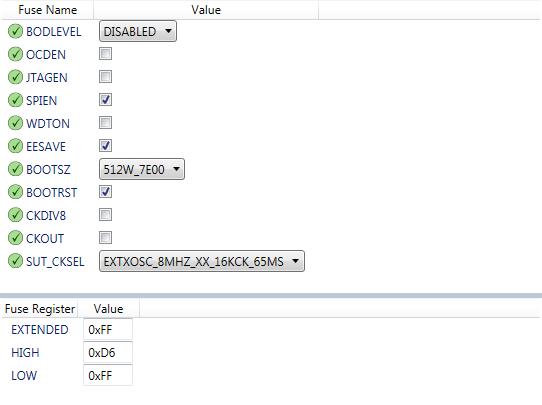
\includegraphics[width=8cm]{content/pictures/Fusebits/fusebits_atmelstudio.png}
\caption{Fuse-Bits im Atmel Studio (ATMega-664P)}
\label{fuses-graf}
\end{figure}

Weitere Hinweise zu den Fuse-Einstellungen gibt es auf mikrocontroller.net
\url{http://www.mikrocontroller.net/articles/AVR_Fuses}.
Eine Website die eine einfache grafische Konfiguration der Fuse-Bits ermöglicht
gibt es bei engbedded.com \url{http://www.engbedded.com/fusecalc/}

